\definecolor{nicegreen}{RGB}{146,208,80}
\definecolor{niceblue}{RGB}{0,176,240}



\part{Continuous Delivery}

\begin{frame}{Agenda}
\begin{itemize}
	\item Continuous Delivery
	\item Delivery Pipeline
	\item Automatic Versioning
	\item Deployment Variants
\end{itemize}
\end{frame}

\begin{frame}{Classic Delivery vs. Continuous Delivery}
\begin{table}[]
\centering

\label{my-label}
\begin{tabular}{@{}cc@{}}
\toprule
\rowcolor[HTML]{EFEFEF} 
\emph{Classic} Delivery  & \emph{Continuous} Delivery\\ \midrule
Big Bang release & No planned release \\
Long development phases  & ``Just in time'' development \\
Manual, many involved parties & Team is accountable\\
Time consuming, complex, error prone & Validation built in \\
\bottomrule
\end{tabular}
\end{table}
\vfill
\emph{Continuous Delivery} doesn't mean every change is automatically deployed to production \ldots 
It means every commit to \emph{master branch} is proven to be deployable at any time.
\end{frame}

\begin{frame}{Trend and Benefits}{Of short Shipment Cycles and Continuous Delivery}
  \centerline{\includeGraphicsTrendCD{width=\textwidth}}

  \begin{block}{Benefits}
  \begin{itemize}
    \item Less risk!
    \item Faster feedback loop to identify bugs
    \item Faster feedback from customers
  \end{itemize}
  \end{block}
\end{frame}

\begin{frame}{Principles and Methods}
Jez Humble:
\begin{quote}
\textbf{If it hurts, do it more often and bring the pain forward!}
\end{quote}
\vfill
  \begin{itemize}
    \item Keep everything in version control
    \item Everybody is responsible
    \item Create repeatable and reliable process
    \item Automate everything
  \end{itemize}
\end{frame}

\begin{frame}{Deployment Pipeline}{Overview Stages}
  \centerline{
    \includeGraphicsPipeline{height=0.6\textheight}
  }

  \begin{itemize}
    \item Qualifies \emph{each} change through the CD pipeline
    \item Visualizes status of release progress
    \item Build centrally only once (xMake) and share artifact on Nexus
  \end{itemize}
\end{frame}

\begin{frame}{Deployment Pipeline}
  \begin{center}
  \colorlink{https://video.sap.com/media/t/1_xy7t3mdv/39197781}{Demo Video: Continuous Delivery in practice}
  \end{center}
  % Show finished Jenkins-Job, maybe also show whole pipeline
\end{frame}

\begin{frame}{Exercise}
Setup a minimal CD pipeline consisting of two stages with Jenkins
\begin{center}
	\vspace{5mm}
	\includeGraphicsPipelineExercise{width=0.5\textwidth}
	\vspace{3mm}

	\colorlink{https://github.com/ccjavadev/cc-coursematerial/blob/master/ContinuousDelivery/Exercise_Setup_CD_Pipeline.md}{Exercise: Setup CD Pipeline}
\end{center}
\end{frame}

\begin{frame}{Automatic Versioning}{Motivation}
  \begin{itemize}
    \item Each version will only be built \emph{once}
    \item Each successful build is a release-candidate
    \item Build references commit for problem analysis
  \end{itemize}

  \uncover<2->{
  \begin{block}{Example}
    \[
      \alert<3>{\overbrace{2.12.65}^{\textnormal{from POM}}}-\alert<4>{\overbrace{20151113}^{\textnormal{date}}}-\alert<5>{\overbrace{141613}^{\textnormal{time}}}\_\alert<6>{\overbrace{\textnormal{c9b6a75acb447282618ff}\cdots{}}^{\textnormal{git hash}}}
    \]
    \vspace{-3mm}
    \begin{itemize}
      \item \codealt{pom.xml} version \alert<3>{$2.12.65$} as defined by the developers
      \item date \alert<4>{November 13\textsuperscript{th}, 2015}
      \item time \alert<5>{14:16:13}
      \item \alert<6>{hash} of \codealt{git} commit
    \end{itemize}
  \end{block}
  }
\end{frame}

\begin{frame}{Automatic Versioning}{Script Implementation}
    \begin{itemize}
      \item Script used in Commit Stage
      \item At the end of the whole pipeline the commit is tagged as 'RELEASE'
      \item No change pushed back into source repository (e.g.\ \codealt{master})
      \begin{itemize}
         \item Avoids merge conflicts in contrast to Maven Release Plugin
      \end{itemize}
    \end{itemize}

    \vspace{5mm}

    \centerline{
      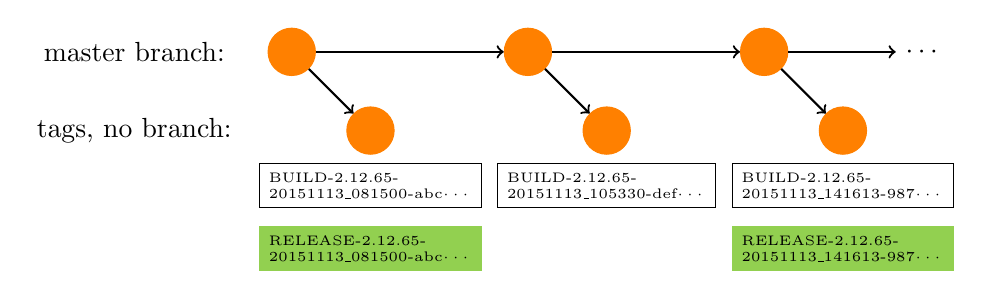
\begin{tikzpicture}[
        commit/.style={circle,draw=orange,fill=orange,minimum height=6mm},
        tag/.style={font=\tiny,rectangle,draw=black,align=left},
        push/.style={draw,->,thick},
      ]
      \node at (-2,0) (Labelmaster) {master branch:};
      \node at (-2,-1) (Labeltags) {tags, no branch:};
      \node[commit] at (0,0) (A) {};
      \node[commit] at (1,-1) (Aversion) {};
%
      \node[commit] at (3,0) (B) {};
      \node[commit] at (4,-1) (Bversion) {};
%
      \node[commit] at (6,0) (C) {};
      \node[commit] at (7,-1) (Cversion) {};
%
      \node[draw=none] at (8,0) (D) {$\cdots$};
%
      \node[tag] at (1,-1.7) (Atag) {BUILD-2.12.65-\\20151113\_081500-abc$\cdots{}$};
      \node[tag,draw=nicegreen,fill=nicegreen] at (1,-2.5) (Ctag) {RELEASE-2.12.65-\\20151113\_081500-abc$\cdots{}$};
%
      \node[tag] at (4,-1.7) (Btag) {BUILD-2.12.65-\\20151113\_105330-def$\cdots{}$};
%
      \node[tag] at (7,-1.7) (Ctag) {BUILD-2.12.65-\\20151113\_141613-987$\cdots{}$};
      \node[tag,draw=nicegreen,fill=nicegreen] at (7,-2.5) (Ctag) {RELEASE-2.12.65-\\20151113\_141613-987$\cdots{}$};
%
      \path[push] (A) -- (B);
      \path[push] (A) -- (Aversion);
      \path[push] (B) -- (C);
      \path[push] (B) -- (Bversion);
      \path[push] (C) -- (D);
      \path[push] (C) -- (Cversion);
    \end{tikzpicture}
    }
\vfill
\uncover<2->{
	Manually change version in \codealt{pom.xml}: e.g.\ for incompatible API changes
}
\end{frame}

\begin{frame}{Blue-Green Deployment}
  \begin{itemize}
    \item \textbf{Goal:} Zero downtime while deploying regularly
    \item Temporarily serve requests with both old and new version
  \end{itemize}

  \begin{block}{Example for \codealt{https://app.sap.com}}   %https://bulletinboard-ads.cfapps.sap.hana.ondemand.com
  \begin{columns}
    \begin{column}{0.65\textwidth}
    \begin{enumerate}
      \item \alert<2>{deploy new version as \codealt{GREEN} app with \codealt{tmpapp} route \\ \codealt{cf push GREEN -n tmpapp}}
      \item \alert<3>{add route to new version\\ \codealt{cf map-route GREEN sap.com -n app}}
      \item \alert<4>{remove route from old version\\ \codealt{cf unmap-route BLUE sap.com -n app}}
      \item \alert<5>{undeploy old version}
      \end{enumerate}
    \end{column}
    \begin{column}{0.3\textwidth}

      \begin{tikzpicture}[->,
        body/.style={star,minimum width=20pt,fill=black},
        head/.style={circle,minimum width=8pt,fill=black},
        desc/.style={rectangle,draw=black},
        app/.style={rectangle,draw=black,minimum width=20pt,minimum height=20pt},
      ]
      \node[head] at (0,0.25) (UserHead) {};
      \node[body] at (0,0) (UserBody) {};
      \node[desc] at (0,-1) (Host) {\codealt{app.sap.com}};
      \node[desc] at (0,-2) (Router) {CF Router};
      \visible<-4>{\node[app,fill=niceblue] at (0,-3) (AppsBlue) {};}
      \visible<2->{\node[app,fill=nicegreen] at (1,-3) (AppsGreen) {};}
      \path[draw,thick] (UserBody) -- (Host);
      \path[draw,thick] (Host) -- (Router);
      \visible<1-3>{\path[draw,thick] (Router) -- (AppsBlue);}
      \visible<3->{\path[draw,thick] (Router) -- (AppsGreen);}
    \end{tikzpicture}
     
    \end{column}
  \end{columns}
  \end{block}
  \footnotesize{\colorlink{https://docs.cloudfoundry.org/devguide/deploy-apps/blue-green.html}{Blue-Green Deployment with CF}}
\end{frame}

\begin{frame}{Canary Deployment}
  \begin{itemize}
    \item \textbf{Goal:} Controlled release of new version to a subgroup of users
    \item Serve only a fraction of requests with new version
    \item Prerequisite: Router needs to be configurable\newline
e.g. which user / how many users should be routed to new version?
  \end{itemize}

  \begin{block}{Example for \codealt{https://app.sap.com}}
  \begin{columns}
    \begin{column}{0.65\textwidth}
    \begin{enumerate}
      \item \alert<2>{route some requests to new version}
      \item \alert<3>{closely monitor new version}
      \item \alert<4>{if OK, increase traffic to new version}
      \end{enumerate}
    \end{column}
    \begin{column}{0.3\textwidth}

	    \begin{tikzpicture}[->,
	      body/.style={star,minimum width=20pt,fill=black},
	      head/.style={circle,minimum width=8pt,fill=black},
	      desc/.style={rectangle,draw=black},
	      app/.style={rectangle,draw=black,minimum width=20pt,minimum height=20pt},
	    ]
	    \node[head] at (0,0.25) (UserHead) {};
	    \node[body] at (0,0) (UserBody) {};
	    \node[desc] at (0,-1) (Host) {\codealt{app.sap.com}};
	    \node[desc] at (0,-2) (Router) {Router};
	%
	    \visible<-1>{\node[app,fill=niceblue] at (1,-3) (AppsBlueA) {};}
	    \visible<-3>{\node[app,fill=niceblue] at (0,-3) (AppsBlueB) {};}
	    \visible<-3>{\node[app,fill=niceblue] at (-1,-3) (AppsBlueC) {};}
	%
	    \visible<2->{\node[app,fill=nicegreen] at (1,-3) (AppsGreenA) {};}
	    \visible<4->{\node[app,fill=nicegreen] at (0,-3) (AppsGreenB) {};}
	    \visible<4->{\node[app,fill=nicegreen] at (-1,-3) (AppsGreenC) {};}
	%
	    \path[draw,thick] (UserBody) -- (Host);
	    \path[draw,thick] (Host) -- (Router);
	%
	    \visible<-1>{\path[draw,thick] (Router) -- (AppsBlueA.north);}
	    \visible<-3>{\path[draw,thick] (Router) -- (AppsBlueB.north);}
	    \visible<-3>{\path[draw,thick] (Router) -- (AppsBlueC.north);}
	%
	    \visible<2->{\path[draw,thick] (Router) -- (AppsGreenA.north);}
	    \visible<4->{\path[draw,thick] (Router) -- (AppsGreenB.north);}
	    \visible<4->{\path[draw,thick] (Router) -- (AppsGreenC.north);}
	  \end{tikzpicture}
    \end{column}
  \end{columns}
  \end{block}
\end{frame}

\begin{frame}{Corporate Requirements and Product Standards}{Still Relevant for Cloud Delivery Channels}
\begin{block}{Corporate Requirements (\colorlink{https://portal.wdf.sap.corp/go/corporaterequirements}{link})}
	\begin{itemize}
		\item Rules to protect SAP as a company from material damage [mandatory for all products]
	\end{itemize}
\end{block}

\begin{block}{Product Standards (PS) (\colorlink{https://portal.wdf.sap.corp/go/productstandards}{link})} 
	\begin{itemize}
		\item Define software qualities to enable SAP‘s business model. 
		\newline[\textbf{Security Product Standard} mandatory for all products]. 
		\item Product Owner responsible for the level of PS compliance.  
		\item The deviations and non-applicability need to be maintained in \colorlink{https://ifp.wdf.sap.corp/prs}{Sirius}. 
	\end{itemize}
\end{block}
\end{frame}

\begin{frame}{Corporate Requirements and Product Standards}{Still Relevant for Cloud Delivery Channels}

%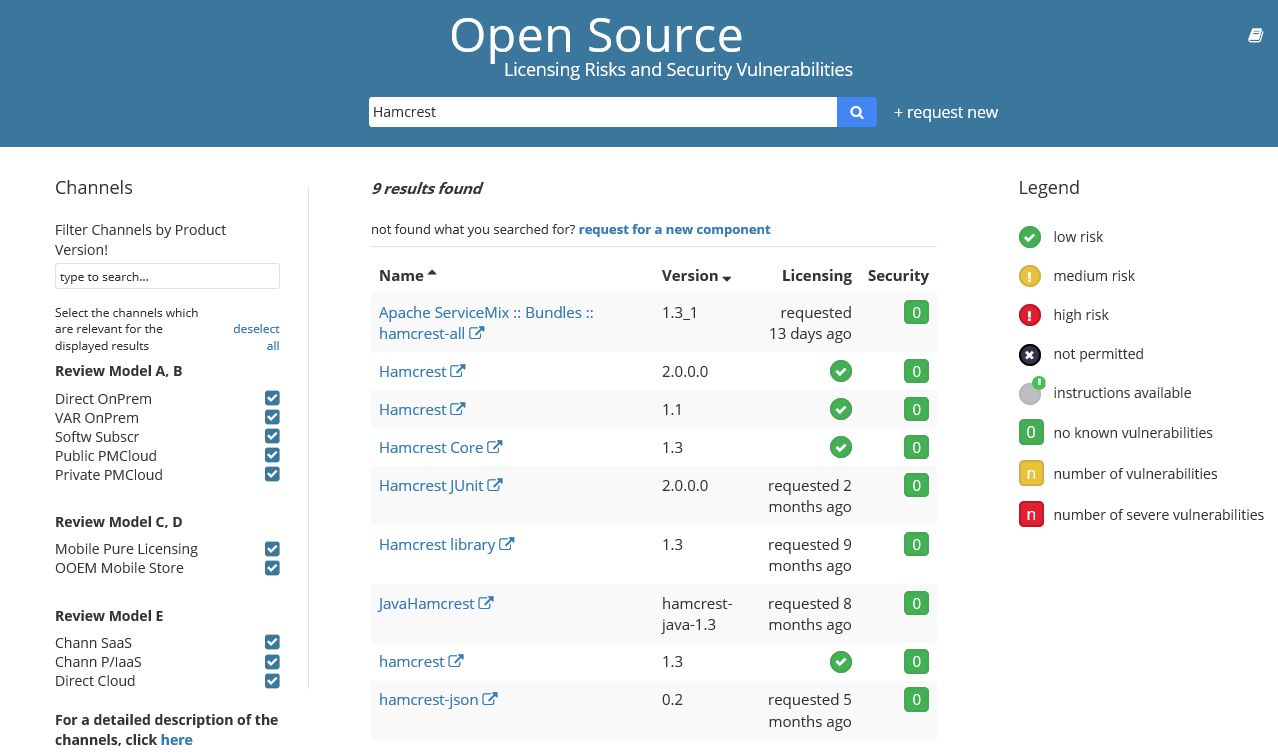
\includegraphics[height=0.35\textheight]{../ContinuousDelivery/images/OpenSourceApi}
%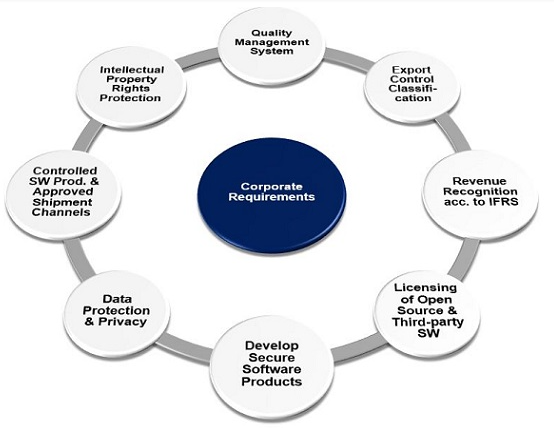
\includegraphics[height=0.35\textheight]{../ContinuousDelivery/images/CorporateRequirementsCircle.png}
%\vfill

\scriptsize%small
 \begin{columns}
    \begin{column}{0.35\textwidth}
	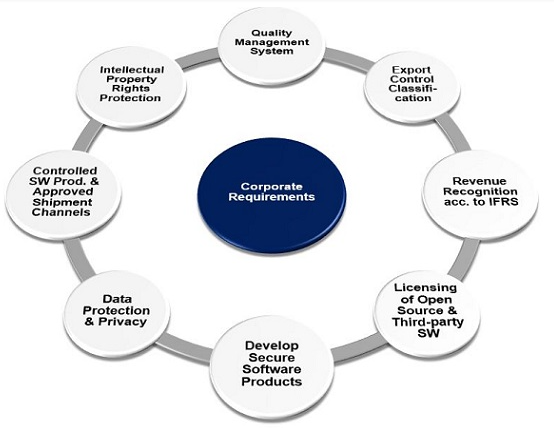
\includegraphics[width=\textwidth]{../ContinuousDelivery/images/CorporateRequirementsCircle}
	\vspace{5mm}
	\\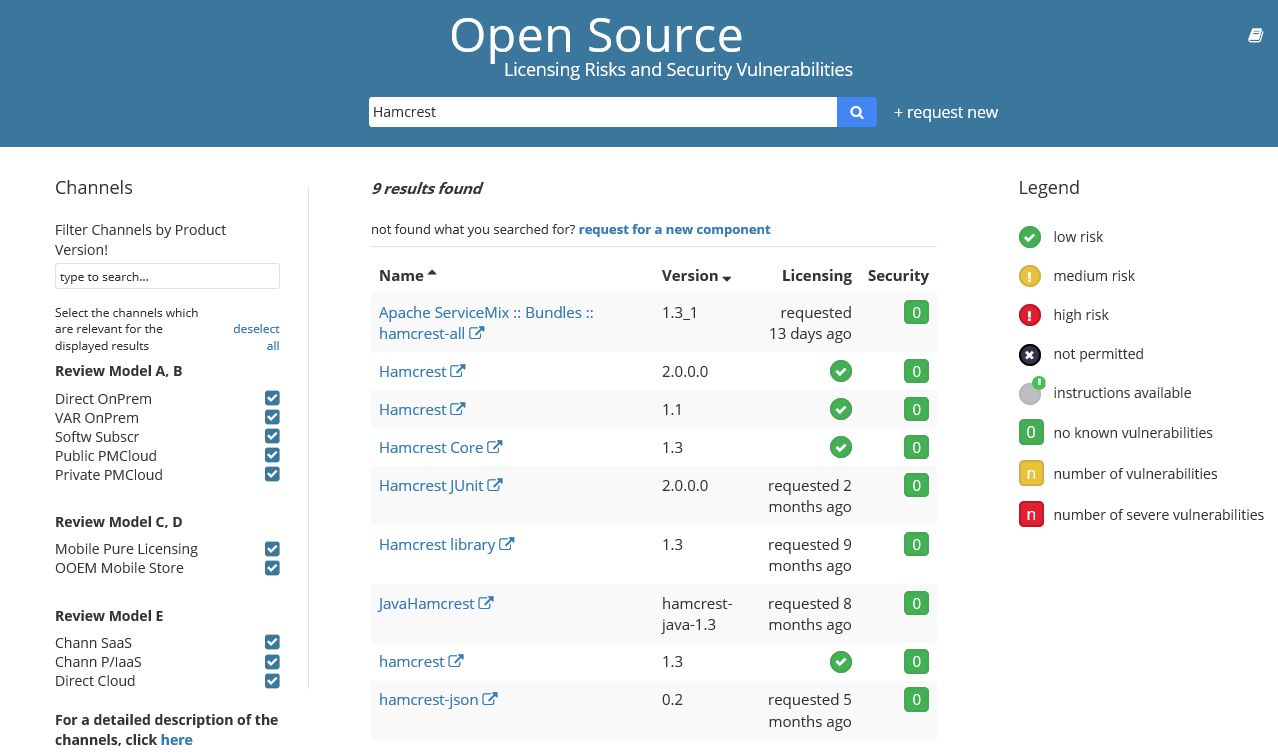
\includegraphics[width=\textwidth]{../ContinuousDelivery/images/OpenSourceApi}
    \end{column}
    \begin{column}{0.6\textwidth}
  	\begin{itemize}
 	   \item \textbf{ECCN} - any Crypto usage in your code / libraries?
           \item \textbf{Licencing} of \colorlink{https://open-source.mo.sap.corp/}{Open Source} and Third-Party Software clarified?\\
    		Risk is evaluated once per library/component and per delivery channel.
	   \item \textbf{Security Scans} - done for your code (e.g. via \emph{Fortify}) \\and used libraries (\colorlink{https://jam4.sapjam.com/groups/XgeUs0CXItfeWyuI4k7lM3/overview_page/2Ocd5GvFueg05eHLqVit9s}{Open Source scans} e.g. \emph{VULAS})
	   \item \textbf{Controlled Software Production} – consider semantic \colorlink{https://sapedia.int.sap/wiki/Semantic_Versioning_and_Incompatibility_in_Continuous_Delivery}{versioning rules} for API compatibility
	   \item \textbf{Intellectual Property} - for your product documented? 
    	   \item \textbf{Traceability} - are new requirements covered by test cases?
       \end{itemize}
	\vspace{2mm}
	\colorlink{https://release-api.mo.sap.corp}{Release API Services} - to fetch data from sources like Sirius, provides information for release decision.
    \end{column}
  \end{columns}
\end{frame}


\begin{frame}{Dynatrace - Professional Monitoring Solution at SAP}
\centerline{
    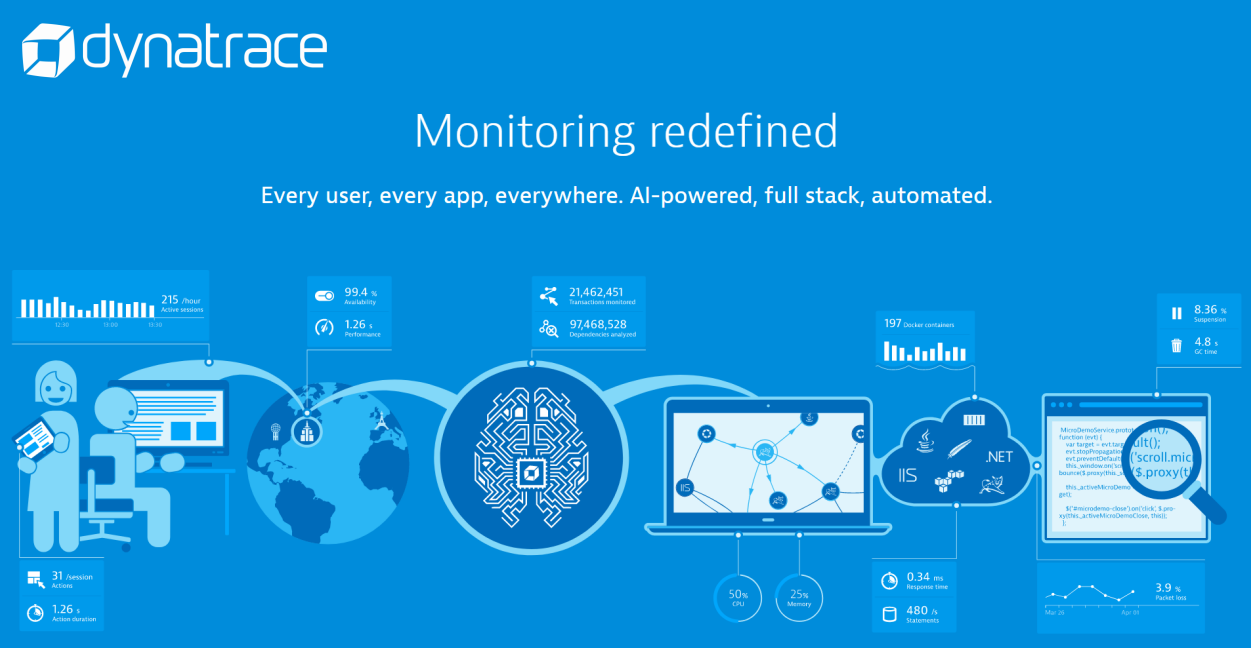
\includegraphics[height=0.35\textheight]{../ContinuousDelivery/images/DynaTrace}
}
\vfill
\scriptsize%small
\textbf{DynaTrace@SAP: \colorlink{https://go.sap.corp/apm}{https://go.sap.corp/apm}}
\begin{itemize}
    \item End-to-end monitoring of application performance: from end user’s browser to the deepest backend systems
    \item Automatic discovery of all components and systems involved in the processing of requests
    \item Infrastructure monitoring, i.e., operative system, network and virtualization
    \item Deep tracing of request processing, down to the single line of code, across all components
    \item Proactive and predictive anomaly detection
    \item Dashboarding and reporting    
\end{itemize}
\end{frame}


\begin{frame}{References}
   \begin{itemize}
	\item \colorlink{https://jam4.sapjam.com/wiki/show/Nz9HvLELqIN8AlvHurIvJS}{Classroom Training: CD and DevOps Training}
	\item \colorlink{https://github.wdf.sap.corp/ContinuousDelivery/jenkins-pipelines}{Ready-to-use Jenkins pipeline templates}
	\item \colorlink{https://jenx.int.sap.hana.ondemand.com/api/}{Jenkins-as-a-Service (JaaS)}
	\item \colorlink{https://account.int.sap.hana.ondemand.com/cockpit\#/home/overview}{SAP Cloud Platform Cockpit}
	\item \colorlink{https://wiki.wdf.sap.corp/wiki/x/lfQrXQ}{ASE Wiki: Continuous Delivery}
	\item \colorlink{http://www.informit.com/articles/article.aspx?p=1621865}{Anatomy of the Deployment Pipeline}
	\item \colorlink{http://continuousdelivery.com/2010/08/continuous-delivery-vs-continuous-deployment/}{Blog: continuous delivery vs continuous deployment (Humble)}
   \end{itemize}
\end{frame}
